\documentclass{standalone}
\usepackage{pgfplots}
\pgfplotsset{compat=newest}
\begin{document}
% same as above with different number of samples
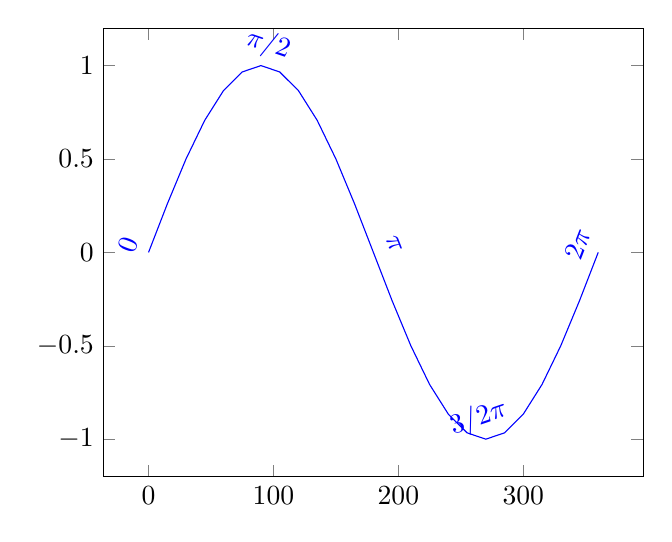
\begin{tikzpicture}
	\begin{axis}
	\addplot[blue,domain=0:360,samples=25] {sin(x)} 
	[every node/.style={yshift=8pt},sloped]
		node[pos=0] {$0$} 
		node[pos=0.25] {$\pi/2$}
		node[pos=0.5] {$\pi$}
		node[pos=0.75] {$3/2\pi$}
		node[pos=1] {$2\pi$}
	;
	\end{axis}
\end{tikzpicture}
\end{document}
